\documentclass[12pt]{article}

\usepackage{graphics}
\usepackage{graphicx}

\setlength{\tabcolsep}{4pt}
\usepackage[ruled,vlined]{algorithm2e}
\usepackage[utf8]{inputenc}
\usepackage[T1]{fontenc}
\usepackage[usenames,dvipsnames]{color}
\usepackage{pgfplots}
\usepackage{a4wide}
\usepackage{afterpage}
\usepackage{amsfonts}
\usepackage{amsmath}
\usepackage{amssymb}
\usepackage{balance}
\usepackage{booktabs}
\usepackage{caption}\DeclareCaptionType{copyrightbox}
\usepackage{enumitem}
\usepackage{epstopdf}
\usepackage{hyperref}
\usepackage{longtable}
\usepackage{multirow}
\usepackage{scalerel}
%\usepackage{subfig}
\usepackage{tabularx}
\usepackage{tikz}
\usepackage{url}
\usepackage{verbatim} 
\usepackage{xcolor}

\usepackage{mathtools}

\usepackage{subfigure}

\include{definitions}

\begin{document}

\newcommand{\citep}[1]{\cite{#1}}
\newcommand{\lipsumcolor}[1]{{\color{blue}\lipsum[#1]}}

\title{P-score: a complementary metric to H-index} 

\author{Jo\~ao Veneroso}
%\affiliation{
%  \institution{CS Dept, UFMG}
%  \city{Belo Horizonte} 
%  \country{Brazil} 
%}
%\email{ueda@dcc.ufmg.br}

\author{Marlon Dias}
%\affiliation{
%  \institution{CS Dept, UFMG}
%  \city{Belo Horizonte} 
%  \country{Brazil} 
%}
%\email{msdias@dcc.ufmg.br}

\author{Berthier Ribeiro-Neto}
%\affiliation{
%  \institution{CS Dept, UFMG \& Google Inc}
%  \city{Belo Horizonte} 
%  \country{Brazil} 
%}
%\email{berthier@dcc.ufmg.br}

\author{Nivio Ziviani}
%\affiliation{
%  \institution{CS Dept, UFMG \& Kunumi}
%  \city{Belo Horizonte} 
%  \country{Brazil} 
%}
%\email{nivio@dcc.ufmg.br}

\author{Edmundo de Souza e Silva}
%\affiliation{
%  \institution{CS Dept, UFRJ}
%  \city{Rio de Janeiro} 
%  \country{Brazil} 
%}
%\email{edmundo@land.ufrj.br}

% If the default list of authors is too long for headers}
%\renewcommand{\shortauthors}{A. Ueda, M. Dias, B. Ribeiro-Neto, N. Ziviani, and E. de Souza e Silva}

% To anonymize:
% \begin{anonsuppress} \end{anonsuppress}

\begin{abstract}
The notion of reputation in academia is critical for taking decisions on research grants, faculty position tenure, 
and research excellence awards. And the notion of reputation is always associated with the publication track 
record of the researcher or research group. Thus, it is important to assess publication track records 
quantitatively. To quantify a publication record, bibliographic metrics are usually adopted. Among these, citation 
based metrics, such as H-indices and citation counts, are quite popular. In this paper we study the correlation between 
P-score, a publication record metric we introduced previously, and H-indices. We show that they are correlated with 
a Kendall-Tau coefficient that exceeds 0.5. Additionally, we noticed that they have important differences. 
We were able to identify publication venues with high H-indices and low P-scores, as well as venues with low 
H-indices and high P-scores. We provide interpretations for these findings and discuss how they can be 
used by research funding councils and committees to better support their funding decisions. 
\end{abstract}

% The code below should be generated by the tool at
% http://dl.acm.org/ccs.cfm
%%%%%%%%%%%%%%%%%%%%%%%%%%%%%%%%%%%%%%%%%%%%%%%%%%%%%%%%%%%%%%%
%\begin{CCSXML}
%<ccs2012>
%<concept>
%<concept_id>10002951.10003317.10003338</concept_id>
%<concept_desc>Information systems~Retrieval models and ranking</concept_desc>
%<concept_significance>500</concept_significance>
%</concept>
%</ccs2012>
%\end{CCSXML}

%\ccsdesc[500]{Information systems~Retrieval models and ranking}
%%%%%%%%%%%%%%%%%%%%%%%%%%%%%%%%%%%%%%%%%%%%%%%%%%%%%%%%%%%%%%%

%\keywords{Academic search, random walks, reputation flows}

\maketitle

\section{Introduction}
\label{sec:introduction}

Academic research evaluation is a topic of interest to universities, research groups,
research funding institutions and the public at large. The evaluation of research
is usually carried out by comparing journals, conferences or papers through the usage of 
academic impact metrics. A popular and moderately effective approach is to compute 
metrics based on the number of citations received by a given piece of research and 
assume that the number of citations is a good proxy for research quality. However,
this approach has multiple shortcomings. 

First, in the evaluation and bibliometrics research communities, citations are understood 
as a measure of attention rather than a proxy for impact or quality. Citations measure 
the attention to a paper of peers in related fields \cite{Loach2015}, not the quality of the 
work produced.

Second, citations can take a long time to happen. To illustrate this, in a recent study that 
looked at first time to citation in a universe of more than a million papers, half the 
papers only received their first citation 20 months or more after they were published \cite{Nane2012}. 

Third, citations are not simple to compute and are not always broadly available, particularly 
at the level of individual researchers. Collecting citation counts requires access to the 
contents of a large number of publications, of which many are not easily available, and 
most authors do not have up to date citation information in their public internet profiles.

Despite these limitations, citation based metrics continue to be a popular approach to
academic research evaluation. Nonetheless, it is desirable to employ alternative and
complementary metrics that tackle the exposed problems without loss of effectiveness.

Academic reputation is an individual or group property strongly associated with 
academic impact. Reputable venues tend to concentrate the most relevant research papers 
because that is how they acquire and keep their good reputations. At the same time, 
reputable authors seek to publish on reputable venues because it gives their 
research more visibility and accreditation. Therefore, a researcher conveys reputation
to a venue proportionally to its own reputation and the reputation of a researcher
is proportional to the reputation of the venues where she or he publishes.
This relationship between authors and venues constitutes a reputation network in which 
authors influence venue reputations and vice versa. 

Pscore is a graph modeling metric that attributes quantitative reputations to venues 
based on the publication patterns of a reference group of researchers without having to
rely on citation information. It deals with the three problems discussed previously. 

First, instead of measuring the amount of researcher attention, Pscore measures reputations,
which is presumably a better proxy for academic impact as was shown by Ribas.

Second, while citations can take years to happen, reputations tend to be steady over 
the time, so the quality of new research can be promptly estimated with pscore by 
simply complementing the reputation flows graph with the newest publication data.

Third, pscore does not require citation data to perform effectively, thus we can avoid
the laborious effort of compiling individual researcher citation information.

The Pscore of computer science venues has shown significant correlation with H-index. Yet, 
there are important cases where the two metrics diverge considerably. Namely, in venues 
that belong to an intersection between different domains and in venues of less popular 
subareas of computer science. These differences appeal to the importance of pscore as a 
complementary metric.

\section{Related Work}\label{sec:related-work}

Quantitative metrics of scientific impact have a long history. An influential approach is
Garfield's Impact Factor (1955) \cite{Garfield1955a}, a journal-level metric that is defined
by the mean number of citations received by articles published in a given journal over a 2-year period. 
Despite being one of the earliest approaches at measuring scientific impact, it has showed remarkable 
survivability. 
Pinski et. al. \cite{Pinski1976} describe several limitations with the metric. Impact factors also suffered 
criticism for being misleading \cite{Nature2016, Saha2003} and for lacking reliable validation from an independent 
audit \cite{Rossner2007}. Riikonen and Vihinen (2008) \cite{Riikonen2008} showed that actual citation 
and publication counts were better predictors of a scientist's contribution than impact factors in a 
study that assessed the scientific contribution of Finnish researchers in biomedicine.

The acceptance rate is another important journal-level metric that attempts to quantify the scientific impact. It
is defined by the proportion of accepted papers relative to the number of submitted papers. Chen et. al. \cite{Chen2010} 
have showed that highly selective conferences (therefore having low acceptance rates) have higher 
scientific impact, measured in terms of the number of citations received by the published papers.

The H-index is an author-level metric proposed by Hirsch (2005) \cite{Hirsch2005}. Since its formulation, it has been 
widely adopted as a measure of invidual scientific research output. An H-index of 
$ h $ means that a researcher has published $ h $ papers that were cited at least $ h $ times.
The H-index takes into account both the number of publications and the number of citations per publication, 
achieving higher values when a researcher obtains a consistently high number of citations over multiple publications. 
The H-index has been criticized for not taking into account field specific citation
statistics \cite{Wendl2007}. The G-index, proposed by Egghe (2006) \cite{Egghe2006}, is a less strict variation 
of the H-index where the score $ g $ is the largest number such that the top $ g $ articles have received at 
least $ g^2 $ citations.

Citation counts and derived metrics are straightforward to calculate, but they represent only a coarse
estimate of academic impact, because they are essentialy popularity measures. Some people are popular but not 
prestigious and vice versa. For example, an author of pulp detectives may sell many books, but may not have earned 
the respect of literary critics \cite{Bollen2006}. Citations from 
prestigious journals are more relevant than citations from peripheral journals, as noted by
Pinski et. al. (1976)  \cite{Pinski1976}. To address this issue, some studies distinguish popularity from 
reputation or prestige with the usage of citation weighting strategies \cite{Ding2011, Yan2011a} or 
PageRank based methods \cite{Bollen2006, Sun2007}. 
Furthermore, Piwowar (2013) \cite{Piwowar2013} noted that citation based metrics are slow, since the 
first citation to a scientific article can take years to happen, concluding that the development of 
alternative metrics to complement citation analysis is not only desirable, but a necessity.
As discussed in \cite{Leydesdorff2009}, each metric has advantages and disadvantages deriving from their 
inherent biases.

Martins et. al. (2009) \cite{Martins2009} proposed a method of assessing the quality of scientific conferences 
through a machine learning classifier that makes use of multiple features in addition to citations.
Gonçalves et al. (2014) \cite{Goncalves2014} quantified the impact of various features on a 
scholar's popularity. They concluded that, even though most of the considered features are strongly correlated 
with popularity, only two features are needed to explain almost all the variation in popularity between different 
researchers: the number of publications and the average quality of the scholar’s publication venues. 

The idea of reputation, without the direct use of citation data, was discussed by Nelakuditi et 
al. \cite{Nelakuditi2011}. They proposed a metric called \textit{peers' reputation} for 
research conferences and journals, which ties the selectivity of the publication venue based upon 
the reputation of its authors' institutions. The proposed metric was shown to be a better indicator 
of the selectivity of a research venue than the acceptance ratio.

In this work, we study the correlation between H-index \cite{Hirsch2005} and \textit{P-score} \cite{Ribas2015a}, a novel
metric for academic reputation. The \textit{P-score} is calculated
with a \textit{reputation flows} model \cite{Ribas2015} instantiantiated in an academic setting.
The \textit{reputation flows} model exploits the transference of reputation among 
entities in order to identify the most reputable ones. Particularly, the reputation flows consist 
of a random walk model where the reputation of a target set of entities is inferred using suitable 
sources of reputation. 

% Regarding ranking researchers according to their expertise or similarity to other
% researchers there are multiple approaches in the literature 
% \cite{Balog2012, Cormode2014, Deng2012, Gollapalli2011, Wu2009}.

\section{P-score: a network-based metric} 
\label{pscore} 

Contrary to citation counting metrics such as the Impact 
Factor~\cite{Garfield1955a, Saha2003, Thomson2017, Balaban2012} and 
H-index~\cite{Benevenuto2016, Bar-Ilan2008, Egghe2008, Bornmann2005, Bornmann2011}, 
P-scores are a graph modeling metric that takes into account 
the relations among researchers, papers they published and their publication venues. They are 
based on a framework of reputation flows we introduced previously \cite{Ribas2015}. Let us review 
them briefly. 

A \emph{reputation graph} in academia is a graph with three node types: (a) {\em reputation sources} representing groups of selected researchers, 
(b) {\em reputation targets} representing venues of interest, and
(c) {\em reputation collaterals} representing entities we want to compare such as research groups and academic 
departments. 
Figure~\ref{fig:overview} provides a generic illustration of our reputation graph and introduces the following 
notation: $S$ is the set of reputation sources, $T$ is the set of reputation targets, and $C$ is the set of reputation collaterals.
We first propagate the reputation of source nodes to target nodes, which allows assigning 
weights to the target nodes. Following, we propagate these weights to the collaterals. 
In here we adopt research groups as source nodes and publication venues as target nodes. 
Further we focus on the weights assigned to the publication venues and do not consider 
potential collaterals of interest (such as individual researchers). 

\begin{figure}[h]
   \centerline{
\includegraphics[scale=0.75]{figures/overview-line}}
   %\centerline{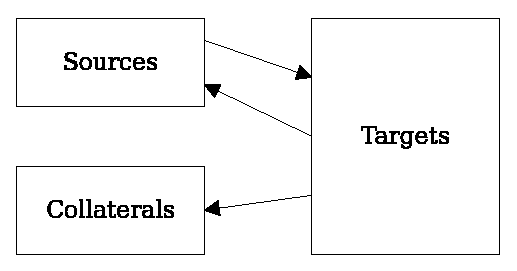
\includegraphics[scale=0.6]{figures/models/overview}}
   \caption{Structure of the reputation graph.}
   \label{fig:overview}
\end{figure}

Our reputation graph for academia can be naturally associated with paper authors, modelled as reputation 
sources, and papers, modelled as reputation targets. 
The interaction between reputation sources and reputation targets is inspired by the 
notion of {\em eigenvalue centrality} in complex 
networks~\cite{Brin1998, Langville2008, Langville2008, Newman2010}. 
In the reputation graph, if we consider only sources and targets, it is easy to identify reputation flows from sources to sources, from sources to targets, from targets to sources, and from targets to targets. These reputation flows can be modeled as a stochastic process. 
In particular, let $P$ be a \emph{right stochastic} %\footnote{A right stochastic matrix is ...} 
matrix of size $(|S|+|T|) \times (|S|+|T|)$ with the following structure: 

\newcommand{\bkt}[1]{ {^{\langle #1 \rangle}} }

\begin{align}\label{eq:newp}
%\[
P =
\left[
\begin{array}{r | r}
(d\bkt{S}) . P\bkt{SS}  & (1-d\bkt{S}) . P\bkt{ST} \\
\hline
(1-d\bkt{T}) . P\bkt{TS}  & (d\bkt{T}) . P\bkt{TT} \\
\end{array}
\right]
%\]
\end{align}
\noindent where each quadrant represents a distinct type of reputation flow, as follows: 

\begin{description}
\item $P\bkt{SS}$: right stochastic matrix of size $|S|\times |S|$ representing the transition probabilities between reputation sources;
\item $P\bkt{ST}$: matrix of size $|S|\times |T|$ representing the transition probabilities from reputation sources to targets;
\item $P\bkt{TS}$: matrix of size $|T|\times |S|$ representing the transition probabilities from reputation targets to sources;
\item $P\bkt{TT}$: right stochastic matrix of size $|T|\times |T|$ representing the transition probabilities between reputation targets.
\end{description}

The parameters $d\bkt{S}$, the fraction of reputation one wants to transfer among the source nodes themselves, 
and $d\bkt{T}$, the fraction of reputation one wants to transfer among the target nodes themselves,
control the relative importance of the reputation sources and targets. 
Assuming that the transition matrix $P$ is ergodic, we can compute the steady state probability of each node and use it as a reputation score. 
More formally, we can write: 
\begin{align}
\label{eq:ggP}
\gamma = \gamma P
\end{align}
\noindent where $\gamma$ is a row matrix with $|S|+|T|$ elements, 
where each row represents the transition probabilities of a node in the set $S\cup T$. 

We should note that, while our network model allows modeling citations in the fourth quadrant, it is possible to compute 
steady state probabilities for the network without consideration to citations. This is accomplished by setting the parameter 
$d\bkt{T} = 0$. 
Thus, it should be clear, in all of our experiments here P-scores 
are computed without taking citations into account. 

%%%%%%%%%%%%% 
\subsection{Reputation Sources}
\label{sec:rep-sources}

The choice of the reputation sources is an important part of the method since its composition has a direct impact in the final rankings. There is no definitive way to make it. This choice depends on what we want to measure. In here we 
use the top CS departments in the US as reputation sources. It is a simple procedure that allows assigning P-scores 
to publication venues, P-scores that 
reflect the publication patterns of top CS departments in the US. 
We then compare how these scores compare with H-indices assigned to the same publication venues. 

One way to determine the top CS departments is to 
adopt the randomization procedure we first described in \cite{Ribas2015b}. A run of that 
procedure works as follows: 
\begin{enumerate}
\item randomly select 10 entities from the set of reputation targets and use them as the set $S$ of reputation sources
\item compute steady state probabilities for all nodes
\item using the steady state probabilities of reputation targets as a score, select the 10 entities with highest scores and use them as a new set $S_{new}$ of reputation sources
\item if $S_{new} \not \equiv S$ then $S \leftarrow S_{new}$ and go back to step 1
\item $S_{auto} \leftarrow S_{new}$ 
\item take $S_{auto}$ as the set of automatically selected reputation sources
\item exit
\end{enumerate}
By applying this randomization procedure 100 times to a set of 126 US graduate programs in Computer Science (CS), 
exactly the same 126 graduate programs considered by NRC in its 2011 evaluation of CS graduate programs 
in the USA \footnote{http://www.nap.edu/rdp/}, we ended up with a subset of 12 CS programs to be considered as reputation sources. 
These are the CS programs that appeared as least once in the set $S_{auto}$ of automatically selected reputation 
sources and they are as follows: 
%%%
\begin{enumerate}
\item Carnegie Mellon University
\item Georgia Institute of Technology
\item Massachusetts Institute of Technology
\item Stanford University
\item University of California-Berkeley
\item University of California-Los Angeles
\item University of California-San Diego
\item University of Illinois at Urbana-Champaign
\item University of Maryland College Park
\item University of Southern California
\item University of Michigan-Ann Arbor
\item Cornell University
\label{list:departments}
\end{enumerate}
%%%

All the 12 departments above are among the top 5th percentile in the ranking produced by NRC. 
This suggests that our recursive procedure is able to take advantage of patterns in the publication 
streams of the various CS departments to determine the most reputable ones in fully automatic fashion.
We further observe that this was done while setting the parameter $d\bkt{T} = 0$. That is, we did 
not use information on citation counts in the model. 

\section{Correlation with H-indices} 
\label{sec:correlation}

The H-index \cite{Hirsch2005} is a composite metric of lifelong scientific contribution that takes 
into account a researcher's productivity and the citation impact of her publications.
A researcher has an H-index value of $ h $ if she has $ h $ publications that have been cited at 
least $ h $ times. For example, if a researcher has published 20 papers that received at least 20 
citations each, then her H-index is 20, assuming that 20 is the highest number for which the 
definition of the H-index holds. A journal's H-index can be computed 
in the same way by considering all publications and their collective citation data over a definite 
period as suggested by Braun et. al. (2006) \cite{Braun2006}.
Since the H-index was proposed in 2005, the original paper by Hirsch \cite{Hirsch2005} was 
cited 7949 times \footnote{According to Google Scholar, up to the end of 2017.} showing the 
metric's popularity.

As any scientific impact metric, the H-index has advantages and disadvantages. 
Some of its advantages are:

\begin{itemize}
\item The simplicity and intuitiveness of its formulation.
\item The longer citation time window when compared to impact factors.
\item The H-index has good predictive power regarding scientific achievement \cite{Bornmann2005, Hirsch2007}.
\end{itemize}

The H-index depends on citations to be calculated, thus it suffers from the 
same problems as other citation-based metrics. Some of the major disadvantages are:

\begin{itemize}
\item The H-index does not distinguish citations from prestigious and peripheral journals, thus 
it measures popularity rather than quality.
\item The time to first citation can be very long.
\item It is not easy to collect all relevant information.
\item The H-index is field-dependent \cite{Wendl2007}.
\item Major sources do not agree about its value. 
\item It allows scientists to rest on their laurels since the number of citations received may increase even if no new paper is published.
\item It is useful for comparing best scientists only. Its power for distinguishing amongst average scientists is not acceptable.
\item It lacks sensitivity to performance changes: it can never decrease and is only weakly sensitive to the number of citations received.
\item The higher the h index the more citations are needed to increase it.11 
\item It means that the difference between higher h index values (25 and 26, for example) is much greater than between lower values (4 and 5, for example).13
\end{itemize}

We propose P-score as a complementary metric to deal with the major problems presented by
citation-based metrics such as the H-index and offer further insight on venue quality.
P-score is a metric of reputation among peers based on the publication pattern of a set of reference 
groups of researchers, the seeds. It differs from other network-based metrics because the venues' reputations 
derive exclusively from the reference set of research groups, better reflecting the actual reputation 
flows. Additionaly, to calculate venue P-scores we do not need citation data, what makes it easier
to obtain than the H-index and avoids the problem of lack of data that arises from the long time to 
first citation.

Our dataset consists of 882 conferences in the area of computer science for which 
the H-index was available on Google Scholar \footnote{https://scholar.google.com.br/}. The
P-score was calculated with data obtained from DBLP \footnote{http://dblp.uni-trier.de/}. 
The reference set of research groups was selected through the randomization process described in 
section \ref{sec:rep-sources}, yielding the 12 departments listed in table \ref{list:departments}.

\begin{figure}[h!]
  \begin{center}
    \begin{tikzpicture}
      \begin{axis}[
          grid=major, % Display a grid
          grid style={dashed,gray!30}, % Set the style
          xlabel=Theoretical Z-Values,
          ylabel=Sample Z-values,
          ymin=-3,
          ymax=10
        ]
        \addplot[blue, only marks, mark size=0.75pt] 
        table[x=column 1,y=column 2,col sep=comma] {data/hindex_normality.csv}; 
        % \legend{Plot}

        \draw[red]
            (axis cs:\pgfkeysvalueof{/pgfplots/xmin},\pgfkeysvalueof{/pgfplots/xmin}) -- 
            (axis cs:\pgfkeysvalueof{/pgfplots/xmax},\pgfkeysvalueof{/pgfplots/xmax});
      \end{axis}
    \end{tikzpicture}
    \caption{H-index Q–Q plot.}
  \end{center}
  \label{fig:hindex_normality}
\end{figure}

\begin{figure}[h!]
  \begin{center}
    \begin{tikzpicture}
      \begin{axis}[
          grid=major, % Display a grid
          grid style={dashed,gray!30}, % Set the style
          xlabel=Theoretical Z-Values,
          ylabel=Sample Z-values,
          ymin=-3,
          ymax=10
        ]
        \addplot[blue, only marks, mark size=0.75pt] 
        table[x=column 1,y=column 2,col sep=comma] {data/pscore_normality.csv}; 
        % \legend{Plot}

        \draw[red]
            (axis cs:\pgfkeysvalueof{/pgfplots/xmin},\pgfkeysvalueof{/pgfplots/xmin}) -- 
            (axis cs:\pgfkeysvalueof{/pgfplots/xmax},\pgfkeysvalueof{/pgfplots/xmax});
      \end{axis}
    \end{tikzpicture}
    \caption{P-score Q–Q plot.}
  \end{center}
  \label{fig:pscore_normality}
\end{figure}

First, we conducted a normality test to verify if P-scores and H-indexes follow normal 
distributions. We plotted Q-Q (quantile-quantile) plots for both metrics comparing the sample
Z-scores for all 882 quantiles to theoretical Z-scores in figures \ref{fig:hindex_normality} 
and \ref{fig:pscore_normality}. The red line is the identity line for which sample Z-scores
and theoretical Z-scores converge. As it is clear from the plots, both distributions are 
significantly skewed, indicating that both P-scores and H-indexes do not follow normal
distributions. This prevents the application of correlation measures such as Pearson's Product 
Moment Correlation in our analysis, since it requires that variables be approximately normally 
distributed. For that reason, we chose the Kendall-Tau coefficient to study the correlation 
between H-index and P-score. It is a measure of rank correlation that assumes a value between
-1 and 1. It is higher when when observations have similar ranks, assuming a value of 1
when all ranks are identical and -1 when they are opposite. A Kendall-Tau close to 0 indicates
that both ranks are completely uncorrelated.

\begin{figure}[h!]
  \begin{center}
    \begin{tikzpicture}
      \begin{axis}[
          grid=major, % Display a grid
          grid style={dashed,gray!30}, % Set the style
          xlabel=P-score ranks,
          ylabel=H-index ranks
        ]
        \addplot[blue, only marks, mark size=0.75pt] 
        table[x=column 1,y=column 2,col sep=comma] {data/pscore_hindex_ranks.csv}; 
      \end{axis}
    \end{tikzpicture}
    \caption{P-score Q–Q plot.}
  \end{center}
  \label{fig:pscore_hindex_ranks}
\end{figure}

Figure \ref{fig:pscore_hindex_ranks} shows the ranks of all data points according to P-score
on the X-axis and H-index on the Y-axis. Points closer to the origin have better scores, therefore
better ranks. The plot shows an evident linear correlation between the ranks that is confirmed
by a very high Kendall-Tau of 0.5200259445, with a p-value smaller than 0.000001, rejecting the null 
hypothesis (that is, the rankings are uncorrelated) by a good margin. 

\section{Assessing conferences in CS}
\label{sec:notifications}

Since P-score and H-index are strongly correlated, most datapoints are clustered close to the identity 
line, showing an apparent agreement between the metrics. However, there are noticeable differences 
particularly in the cases where the P-score rank is high and the H-index rank is low 
(top left corner of figure \ref{fig:pscore_hindex_ranks}) or where the H-index rank is high and the 
P-score rank is low (bottom right corner of figure \ref{fig:pscore_hindex_ranks}). 

We propose a simple strategy to delimit the 3 groups of datapoints: 
\begin{itemize}
\item the center group, consisting of the highly correlated datapoints. Venues that are popular and
prestigious, or venues that are unpopular and unprestigious.
\item the top group, consisting of the ones with a high P-score and low H-index. Venues that are 
prestigous, but not very popular.
\item the bottom group, consisting of the ones with a high H-index and low P-score. Venues that are
popular but not so prestigious.
\end{itemize}

\begin{figure}[h!]
  \begin{center}
    \begin{tikzpicture}
      \begin{axis}[
          grid=major, % Display a grid
          grid style={dashed,gray!30}, % Set the style
          xlabel=P-score ranks,
          ylabel=H-index ranks
          xmin=-100,
          ymin=-100,
          xmax=1000,
          ymax=1000,
        ]
        \draw[red]
            (axis cs:0,0) -- 
            (axis cs:700.207670245,1000);
        \draw[red]
            (axis cs:0,0) -- 
            (axis cs:1000,700.207670245);
        \addplot[blue, only marks, mark size=0.75pt] 
        table[x=column 1,y=column 2,col sep=comma] {data/pscore_hindex_ranks.csv}; 

      \end{axis}
    \end{tikzpicture}
    \caption{P-score Q–Q plot.}
  \end{center}
  \label{fig:cone_strategy}
\end{figure}

\begin{table}[h!]
\centering
 \begin{tabular}{|c c c|} 
 \hline
 Angle & Kendall-Tau & Items in center group \\ 
 \hline
 90 & 0.5003 & 882 \\ 
 80 & 0.5027 & 877 \\ 
 70 & 0.5127 & 862 \\ 
 60 & 0.5304 & 836 \\ 
 50 & 0.5510 & 795 \\ 
 40 & 0.5946 & 734 \\ 
 30 & 0.6334 & 637 \\ 
 20 & 0.7129 & 483 \\ 
 10 & 0.8295 & 281 \\ 
 \hline
 \end{tabular}
 \label{tab:cone_strategy}
\end{table}

The cone strategy consists of two lines crossing at the origin that delimit the boundaries between
the 3 groups. The datapoints become more scattered in lower positions because venues with low reputation
or few citations become increasingly harder to rank because of a lack of signals. The cone strategy
deals with this problem by imposing a softer criterion for the cut off of venues (from the center group) in
lower ranks. Figure \ref{fig:cone_strategy} shows the cone strategy with an angle of 20 degrees
between the boundary lines. Table \ref{tab:cone_strategy} describes the Kendall-Tau values for varying angles
between boundary lines and the number of datapoints in the center group. Eventhough P-score and H-index are
very correlated, there are still differences in rank even for the datapoints that show an agreement between 
metrics. We want to separate the differences that are mostly noise (in the center venues) from the differences
that show a disagreement between metrics (the botttom and top groups). For our further analysis, we employed 
the cone strategy with a 20 degrees angle, because it presents a good trade off between both objectives.

\begin{figure}[h!]
  \begin{center}
    \begin{tikzpicture}
      \begin{axis}[
          grid=major, % Display a grid
          grid style={dashed,gray!30}, % Set the style
          xlabel=P-score ranks,
          ylabel=H-index ranks
          xmin=-100,
          ymin=-100,
          xmax=1000,
          ymax=1000,
        ]
        \draw[red]
            (axis cs:-100,-100) -- 
            (axis cs:700.207670245,1000);
        \draw[red]
            (axis cs:-100,-100) -- 
            (axis cs:1000,700.207670245);
        \addplot[blue, only marks, mark size=0.75pt] 
        table[x=column 1,y=column 2,col sep=comma] {data/pscore_hindex_ranks.csv}; 

      \end{axis}
    \end{tikzpicture}
    \caption{P-score Q–Q plot.}
  \end{center}
  \label{fig:cone_strategy_adapted}
\end{figure}

The cone strategy shown in figure \ref{fig:cone_strategy} imposes a very strict criterion of cut off
for venues close to the origin, such that only venues that are almost over the identity line end up belonging
to the center group. This is not desirable, because even though the ranks for these venues are not 
exactly the same in P-score or H-index, they are roughly in agreement. To sort out this problem
we moved the pivot point where the boundary lines cross to coordinates (-100, -100), achieving a better 
demarcation of the data groups. Figure \ref{fig:cone_strategy_adapted} shows the result.

\begin{table}[h!]
\centering
 \begin{tabular}{|c c c|} 
 \hline
 Conference \\ 
 \hline
 IEEE/RJS International Conference on Intelligent RObots and Systems (IROS) \\
 International Conference on Multimedia Computing and Systems (ICMCS) \\
 Symposium on Information Theory (ISIT) \\
 Conference on Computer Design (ICCD) \\
 IEEE Conference on Decision and Control (CDC) \\
 Conference on Parallel Processing (ICPP) \\
 ACM Symposium on Parallel Algorithms and Architectures (SPAA) \\
 Conference Computational Learning Theory (COLT) \\
 IEEE Wireless Communications and Networking Conference (WCNC) \\
 Workshop on Languages and Compilers for Parallel Computing (LCPC) \\
 IEEE International Symposium on Quality Electronic Design (ISQED) \\
 Workshop on Approximation Algorithms for Combinatorial Optimization (APPROX) \\
 Symposium on Experimental Robotics (ISER) \\
 IEEE Workshop/Winter Conference on Applications of Computer Vision (WACV) \\
 Conference on Intelligent Tutoring Systems (ITS) \\
 Conference on Weblogs and Social Media (ICWSM) \\
 Conference on Artificial Intelligence in Education (AIED) \\
 ACM SIGSPATIAL International Workshop on Advances in Geographic Information Systems (GIS) \\
 IEEE/ACM International Conference on Human-Robot Interaction (HRI) \\
 Canadian Conference on Computational Geometry (CCCG) \\
 ACM Workshop on Hot Topics in Networks (HotNets) \\
 IEEE Communications Society Conference on Sensor, Mesh and Ad Hoc Communications and Networks (SECON) \\
 IEEE-RAS International Conference on Humanoid Robots (Humanoids) \\
 Conference on Computer Communications and Networks (ICCCN) \\
 SIAM Conference on Parallel Processing for Scientific Computing \\
 DG.O (Inter)National Conference on Digital Government Research \\
 Conference on High Performance Computing (HiPC) \\
 Workshop on the Algorithmic Foundations of Robotics (WAFR) \\
 IEEE International Symposium on Biomedical Imaging: From Nano to Macro (ISBI) \\
 IEEE International Conference on Systems, Man and Cybernetics (SMC) \\
 \hline
 \end{tabular}
 \label{tab:top_group}
\end{table}

\begin{table}[h!]
\centering
 \begin{tabular}{|c c c|} 
 \hline
 Conference \\ 
 \hline
 IEEE International Conference on Robotics and Automation (ICRA)
 Conference on Human Factors in Computing Systems (CHI)
 Computer Vision and Pattern Recognition (CVPR)
 AAAI Conference on Artificial Intelligence (AAAI)
 Neural Information Processing Systems (NIPS)
 Design Automation Conference (DAC)
 IEEE International Conference on Acoustics, Speech, and Signal Processing (ICASSP)
 Symposium on the Theory of Computing (STOC)
 IEEE Symposium on Foundations of Computer Science (FOCS)
 Conference of the International Speech Communication Association (INTERSPEECH)
 Conference on Computer Aided Design (ICCAD)
 Joint Conference on Artificial Intelligence (IJCAI)
 ACM-SIAM Symposium on Discrete Algorithms (SODA)
 INFOCOM (IEEE) (INFOCOM)
 Conference on Machine Learning (ICML)
 IEEE International Conference on Image Processing (ICIP)
 Conference on Management of Data (SIGMOD)
 Conference on Software Engineering (ICSE)
 International Parallel (and Distributed) Processing Symposium (IP(D)PS)
 IEEE International Conference on Computer Vision (ICCV)
 IEEE International Conference on Data Engineering (ICDE)
 Meeting of the Association for Computational Linguistics (ACL)
 European Conference on Computer Vision (ECCV)
 Symposium on Computer Architecture (ISCA)
 Knowledge Discovery and Data Mining (KDD)
 Conference on Applications, Technologies, Architectures, and Protocols for Computer Communication (SIGCOMM)
 Supercomputing (SC)
 World Wide Web Conferences (WWW)
 IEEE International Conference on Distributed Computing Systems (ICDCS)
 Design, Automation, and Test in Europe (DATE)
 \hline
 \end{tabular}
 \label{tab:bottom_group}
\end{table}

\begin{table}[h!]
\centering
 \begin{tabular}{|c c c|} 
 \hline
 Conference \\ 
 \hline
 IEEE International Symposium on Circuits and Systems (ISCAS) \\
 Hawaii International Conference on System Sciences (HICSS) \\
 Conference on the Theory and Application of Cryptographic Techniques (EUROCRYPT) \\
 ACM/SIGCOMM Internet Measurement Conference (IMC) \\
 IEEE International Symposium on Wearable Computers (ISWC) \\
 ASIACRYPT \\
 Intelligent Systems in Molecular Biology (ISMB) \\
 Conference on Tools and Algorithms for Construction and Analysis of Systems (TACAS) \\
 ACM Interational Symposium on Mobile Ad Hoc Networking and Computing (MobiHoc) \\
 IEEE Vehicular Technology Conference (VTC) \\
 Computer Security Applications Conference (ACSAC) \\
 Pacific Symposium on Biocomputing (PSB) \\
 Genetic and Evolutionary Computation Conference (GECCO) \\
 IEEE International Conference on Web Services (ICWS) \\
 European Symposium on Programming (ESOP) \\
 European Conference on Artificial Intelligence (ECAI) \\
 Adaptive Agents and Multi-Agent Systems (AAMAS) \\
 Conference on Theory and Practice of Public Key Cryptography (PKC) \\
 Conference on Principles and Practice of Constraint Programming (CP) \\
 Society for Music Information Retrieval Conference (ISMIR) \\
 Conference on Information Systems (ICIS) \\
 Euromicro Conference on Real-Time Systems (ECRTS) \\
 Fast Software Encryption Workshop (FSE) \\
 IEEE International Symposium on Personal, Indoor and Mobile Radio Communications (PIMRC) \\
 GI-Jahrestagung \\
 ACM Symposium on Access Control Models and Technologies (SACMAT) \\
 Pacific Conference on Computer Graphics and Applications (PG) \\
 Discovery Science \\
 IEEE International Conference on Peer-to-Peer Computing (P2P) \\
 ACM/IEEE International Conference on Model Driven Engineering Languages and Systems (MoDELS) \\
 \hline
 \end{tabular}
 \label{tab:bottom_group}
\end{table}

With this final demarcation strategy, the top group ended up with 127 venues, the 
center group with 616 venues, and the bottom group with 139 venues. Following, we present 
interpretations for these findings.
The top group consists of venues with a high P-score and low H-index, or high prestige 
and low popularity, the top 30 conferences in this group (by P-score) are presented in
table \ref{tab:top_group}. These venues belong to less popular sub areas in computer science.
The bottom group consists of venues with a low P-score and high H-index, or low prestige 
and high popularity, the top 30 conferences in this group (by P-score) are presented in
table \ref{tab:bottom_group}. These venues belong to less popular sub areas in computer science.







\section{Conclusions}\label{sec:conclusions}

ZZZ Rewrite entirely.

\begin{comment}
\begin{acks}

ZZZ Thank scholarships by CAPES and CNPq.

\end{acks}
\end{comment}
%% To fill space (Ueda)
\section*{ACKNOWLEDGEMENTS}
Omitted for blind review.

%\bibliographystyle{ACM-Reference-Format}
\bibliographystyle{abbrv}
\bibliography{pscore_correlation}

\end{document}

